\documentclass[10pt]{article}
\usepackage[T1]{fontenc}

% Document Details
\newcommand{\CLASS}{AMATH 585}
\newcommand{\assigmentnum}{Assignment 2}

\usepackage[margin = 1.15in, top = 1.25in, bottom = 1.in]{geometry}

\usepackage{titling}
\setlength{\droptitle}{-6em}   % This is your set screw
\date{}
\renewcommand{\maketitle}{
	\clearpage
	\begingroup  
	\centering
	\LARGE \sffamily\textbf{\CLASS} \Large \assigmentnum\\[.8em]
	\large Tyler Chen\\[1em]
	\endgroup
	\thispagestyle{empty}
}
 % Title Styling
\usepackage{tocloft}
\renewcommand{\cfttoctitlefont}{\Large\sffamily\bfseries}
\renewcommand{\cftsecfont}{\normalfont\sffamily\bfseries}
\renewcommand{\cftsubsecfont}{\normalfont\sffamily}
\renewcommand{\cftsubsubsecfont}{\normalfont\sffamily}

\makeatletter
\let\oldl@section\l@section
\def\l@section#1#2{\oldl@section{#1}{\sffamily\bfseries#2}}

\let\oldl@subsection\l@subsection
\def\l@subsection#1#2{\oldl@subsection{#1}{\sffamily#2}}

\let\oldl@subsubsection\l@subsubsection
\def\l@subsubsection#1#2{\oldl@subsubsection{#1}{\sffamily#2}}
 % General Styling


\usepackage{enumitem}

% Figures
\usepackage{subcaption}

% TikZ and Graphics
\usepackage{tikz, pgfplots}
\pgfplotsset{compat=1.12}
\usetikzlibrary{patterns,arrows}
\usepgfplotslibrary{fillbetween}

\usepackage{pdfpages}
\usepackage{adjustbox}

\usepackage{lscape}
\usepackage{titling}
\usepackage[]{hyperref}


% Header Styling
\usepackage{fancyhdr}
\pagestyle{fancy}
\lhead{\sffamily \CLASS}
\rhead{\sffamily Chen \textbf{\thepage}}
\cfoot{}

% Paragraph Styling
\setlength{\columnsep}{1cm}
\setlength{\parindent}{0pt}
\setlength{\parskip}{5pt}
\renewcommand{\baselinestretch}{1}

% TOC Styling
\usepackage{tocloft}
\iffalse
\renewcommand{\cftsecleader}{\cftdotfill{\cftdotsep}}

\renewcommand\cftchapafterpnum{\vskip6pt}
\renewcommand\cftsecafterpnum{\vskip10pt}
\renewcommand\cftsubsecafterpnum{\vskip6pt}

% Adjust sectional unit title fonts in ToC
\renewcommand{\cftchapfont}{\sffamily}
\renewcommand{\cftsecfont}{\bfseries\sffamily}
\renewcommand{\cftsecnumwidth}{2em}
\renewcommand{\cftsubsecfont}{\sffamily}
\renewcommand{\cfttoctitlefont}{\hfill\bfseries\sffamily\MakeUppercase}
\renewcommand{\cftaftertoctitle}{\hfill}

\renewcommand{\cftchappagefont}{\sffamily}
\renewcommand{\cftsecpagefont}{\bfseries\sffamily}
\renewcommand{\cftsubsecpagefont}{\sffamily}
\fi
 % General Styling
% Code Display Setup
\usepackage{listings,lstautogobble}
\usepackage{lipsum}
\usepackage{courier}
\usepackage{catchfilebetweentags}

\lstset{
	basicstyle=\small\ttfamily,
	breaklines=true, 
	frame = single,
	rangeprefix=,
	rangesuffix=,
	includerangemarker=false,
	autogobble = true
}


\usepackage{algorithmicx}
\usepackage{algpseudocode}

\newcommand{\To}{\textbf{to}~}
\newcommand{\DownTo}{\textbf{downto}~}
\renewcommand{\algorithmicdo}{\hspace{-.2em}\textbf{:}}
 % Code Display Setup
% AMS MATH Styling
\usepackage{amsmath, amssymb}
\newcommand{\qed}{\hfill\(\square\)}

%\newtheorem*{lemma}{Lemma} 
%\newtheorem*{theorem}{Theorem}
%\newtheorem*{definition}{Definition}
%\newtheorem*{prop}{Proposition}
%\renewenvironment{proof}{{\bfseries Proof.}}{}


% mathcal
\newcommand{\cA}{\ensuremath{\mathcal{A}}}
\newcommand{\cB}{\ensuremath{\mathcal{B}}}
\newcommand{\cC}{\ensuremath{\mathcal{C}}}
\newcommand{\cD}{\ensuremath{\mathcal{D}}}
\newcommand{\cE}{\ensuremath{\mathcal{E}}}
\newcommand{\cF}{\ensuremath{\mathcal{F}}}
\newcommand{\cG}{\ensuremath{\mathcal{G}}}
\newcommand{\cH}{\ensuremath{\mathcal{H}}}
\newcommand{\cI}{\ensuremath{\mathcal{I}}}
\newcommand{\cJ}{\ensuremath{\mathcal{J}}}
\newcommand{\cK}{\ensuremath{\mathcal{K}}}
\newcommand{\cL}{\ensuremath{\mathcal{L}}}
\newcommand{\cM}{\ensuremath{\mathcal{M}}}
\newcommand{\cN}{\ensuremath{\mathcal{N}}}
\newcommand{\cO}{\ensuremath{\mathcal{O}}}
\newcommand{\cP}{\ensuremath{\mathcal{P}}}
\newcommand{\cQ}{\ensuremath{\mathcal{Q}}}
\newcommand{\cR}{\ensuremath{\mathcal{R}}}
\newcommand{\cS}{\ensuremath{\mathcal{S}}}
\newcommand{\cT}{\ensuremath{\mathcal{T}}}
\newcommand{\cU}{\ensuremath{\mathcal{U}}}
\newcommand{\cV}{\ensuremath{\mathcal{V}}}
\newcommand{\cW}{\ensuremath{\mathcal{W}}}
\newcommand{\cX}{\ensuremath{\mathcal{X}}}
\newcommand{\cY}{\ensuremath{\mathcal{Y}}}
\newcommand{\cZ}{\ensuremath{\mathcal{Z}}}

% mathbb
\usepackage{bbm}
\newcommand{\bOne}{\ensuremath{\mathbbm{1}}}

\newcommand{\bA}{\ensuremath{\mathbb{A}}}
\newcommand{\bB}{\ensuremath{\mathbb{B}}}
\newcommand{\bC}{\ensuremath{\mathbb{C}}}
\newcommand{\bD}{\ensuremath{\mathbb{D}}}
\newcommand{\bE}{\ensuremath{\mathbb{E}}}
\newcommand{\bF}{\ensuremath{\mathbb{F}}}
\newcommand{\bG}{\ensuremath{\mathbb{G}}}
\newcommand{\bH}{\ensuremath{\mathbb{H}}}
\newcommand{\bI}{\ensuremath{\mathbb{I}}}
\newcommand{\bJ}{\ensuremath{\mathbb{J}}}
\newcommand{\bK}{\ensuremath{\mathbb{K}}}
\newcommand{\bL}{\ensuremath{\mathbb{L}}}
\newcommand{\bM}{\ensuremath{\mathbb{M}}}
\newcommand{\bN}{\ensuremath{\mathbb{N}}}
\newcommand{\bO}{\ensuremath{\mathbb{O}}}
\newcommand{\bP}{\ensuremath{\mathbb{P}}}
\newcommand{\bQ}{\ensuremath{\mathbb{Q}}}
\newcommand{\bR}{\ensuremath{\mathbb{R}}}
\newcommand{\bS}{\ensuremath{\mathbb{S}}}
\newcommand{\bT}{\ensuremath{\mathbb{T}}}
\newcommand{\bU}{\ensuremath{\mathbb{U}}}
\newcommand{\bV}{\ensuremath{\mathbb{V}}}
\newcommand{\bW}{\ensuremath{\mathbb{W}}}
\newcommand{\bX}{\ensuremath{\mathbb{X}}}
\newcommand{\bY}{\ensuremath{\mathbb{Y}}}
\newcommand{\bZ}{\ensuremath{\mathbb{Z}}}

% alternative mathbb
\newcommand{\NN}{\ensuremath{\mathbb{N}}}
\newcommand{\RR}{\ensuremath{\mathbb{R}}}
\newcommand{\CC}{\ensuremath{\mathbb{C}}}
\newcommand{\ZZ}{\ensuremath{\mathbb{Z}}}
\newcommand{\EE}{\ensuremath{\mathbb{E}}}
\newcommand{\PP}{\ensuremath{\mathbb{P}}}
\newcommand{\VV}{\ensuremath{\mathbb{V}}}
\newcommand{\cov}{\ensuremath{\text{Co}\VV}}
% Math Commands

\newcommand{\st}{~\big|~}
\newcommand{\stt}{\text{ st. }}
\newcommand{\ift}{\text{ if }}
\newcommand{\thent}{\text{ then }}
\newcommand{\owt}{\text{ otherwise }}

\newcommand{\norm}[1]{\left\lVert#1\right\rVert}
\newcommand{\snorm}[1]{\lVert#1\rVert}
\newcommand{\ip}[1]{\ensuremath{\left\langle #1 \right\rangle}}
\newcommand{\pp}[3][]{\frac{\partial^{#1}#2}{\partial #3^{#1}}}
\newcommand{\dd}[3][]{\frac{\d^{#1}#2}{\d #3^{#1}}}
\renewcommand{\d}{\ensuremath{\mathrm{d}}}

\newcommand{\indep}{\rotatebox[origin=c]{90}{$\models$}}




 % Math shortcuts
% Problem
\usepackage{floatrow}

\newenvironment{problem}[1][]
{\pagebreak
\noindent\rule{\textwidth}{1pt}\vspace{0.25em}
{\sffamily \textbf{#1}}
\par
}
{\par\vspace{-0.5em}\noindent\rule{\textwidth}{1pt}}

\newenvironment{solution}[1][]
{{\sffamily \textbf{#1}}
\par
}
{}

 % Problem Environment

\newcommand{\note}[1]{\textcolor{red}{\textbf{Note:} #1}}

\hypersetup{
   colorlinks=true,       % false: boxed links; true: colored links
   linkcolor=violet,          % color of internal links (change box color with linkbordercolor)
   citecolor=green,        % color of links to bibliography
   filecolor=magenta,      % color of file links
   urlcolor=cyan           % color of external links
}


\begin{document}
\maketitle


\begin{problem}[Problem 1  (Inverse matrix and Green's functions)]
\begin{enumerate}
    \item[(a)] Write out the \(5\times 5\) matrix \(A\) from (2.43) for the boundary value problem \(u''(x)=f(x)\) with \(u(0)=u(1)=0\) for  \(h = 0.25\).
    \item[(b)] Write out the \(5\times 5\) inverse matrix \(A^{-1}\) explicitly for this problem.
    \item[(c)] If \(f(x)=x\), determine the discrete approximation to the solution of the boundary value problem on this grid and sketch this solution and the five Green's functions whose sum gives this solution.
\end{enumerate}
\end{problem}

\begin{solution}[Solution]

\begin{enumerate}
    \item[(a)] We have,
        \begin{align*}
            A=
            \dfrac{1}{h^2}\left[\begin{array}{rrrrr}
                h^2 & 0 \\
                1 & -2 & 1 \\
                & 1 & -2 & 1 \\
                && 1 & -2 & 1 \\
                &&& 0 & h^2 
            \end{array}\right]
            =
            \left[\begin{array}{rrrrr}
                1 & 0 \\
                16 & -32 & 16 \\
                & 16 & -32 & 16 \\
                && 16 & -32 & 16 \\
                &&& 0 & 1
            \end{array}\right]
        \end{align*}
    \item[(b)]
        Since \( h=1/4 \) we have,
        \begin{align*}
            x_0 = 0 && x_1 = 1/4 && x_2 = 2/4 && x_3 = 3/4 && x_4 = 1
        \end{align*}

        In the first and last columns we have,
        \begin{align*}
            B_{i,0} = 1-x_i && B_{i,4} = x_i
        \end{align*}

        In the middle columns we have,
        \begin{align*}
            B_{i,j} = h G(x_i;x_j) = \begin{cases}
                h(x_j-1)x_i, & i=0,1,\ldots,j \\
                h(x_i-1)x_j, & i=j, j+1, \ldots, m+1
            \end{cases}
        \end{align*}
        
        Thus,
        \begin{align*}
            B &= 
            \left[\begin{array}{rrrrr}
                1-x_0 & h(x_1-1)x_0 & h(x_2-1)x_0 & h(x_3-1)x_0 & x_0 \\
                1-x_1 & h(x_1-1)x_1 & h(x_2-1)x_1 & h(x_3-1)x_1 & x_1 \\
                1-x_2 & h(x_2-1)x_1 & h(x_2-1)x_2 & h(x_3-1)x_2 & x_2 \\
                1-x_3 & h(x_3-1)x_1 & h(x_3-1)x_2 & h(x_3-1)x_3 & x_3 \\
                1-x_4 & h(x_4-1)x_1 & h(x_4-1)x_2 & h(x_4-1)x_3 & x_4
            \end{array}\right]
            \\ &= 
            \left[\begin{array}{rrrrr}
                1   & 0 & 0 & 0 & 0 \\
                3/4 & -3/64 & -1/32 & -1/64 & 1/4 \\
                1/2 & -1/32 & -1/16 & -1/32 & 1/2 \\
                1/4 & -1/64 & -1/32 & -3/64 & 3/4 \\
                0   & 0 & 0 & 0 & 1
            \end{array}\right]
        \end{align*}

        We easily verify that \( B=A^{-1} \) using Mathematica.

    \item[(c)]
        We have,
        \begin{align*}
            F = \left[\begin{array}{r}
                \alpha \\ x_1 \\ x_2 \\ x_3 \\ \beta
            \end{array}\right]
            = \left[\begin{array}{r}
                0 \\ 1/4 \\ 1/2 \\ 3/4 \\ 0 
            \end{array}\right]
        \end{align*}

        We solve \( AU = F \), where \( U = [U_0, ..., U_{4}]^T \) yielding,
        \begin{align*}
            U = \alpha B_0 + \beta B_4 + \sum_{j=1}^{3}x_jB_j = \sum_{j=1}^{3}x_jB_j
           = \left[\begin{array}{r}
                0 \\ -5/128 \\ -1/16 \\ -7/128 \\ 0
            \end{array}\right]
        \end{align*}

       Figure~\ref{g1} shows the 5 greens functions corresponding to the 5 points in \( F \). Figure~\ref{g2} shows the Green's functions after they have been scaled using the coefficients of \( F \). Figure~\ref{g3} shows the sum of the scaled Green's functions along with the actual solution \( u(x) = (x^3-x)/6 \).
        \begin{figure}[H]\centering
            \begin{subfigure}{.49\textwidth}\centering
                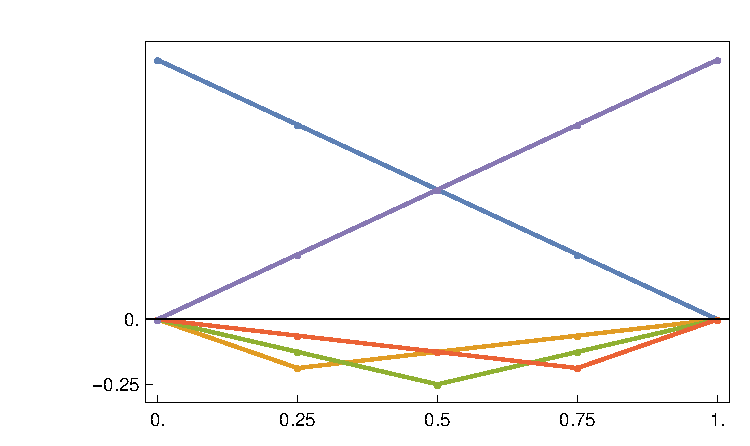
\includegraphics[width=\textwidth]{img/g1.pdf}
                \caption{Green's functions}
                \label{g1}
            \end{subfigure}
            \begin{subfigure}{.49\textwidth}\centering
                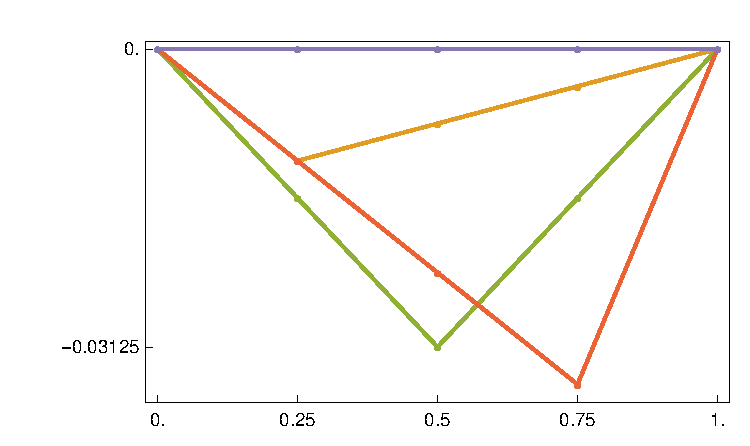
\includegraphics[width=\textwidth]{img/g2.pdf}
                \caption{Green's functions with scaled axes}
                \label{g2}
            \end{subfigure}
            \begin{subfigure}{.49\textwidth}\centering
                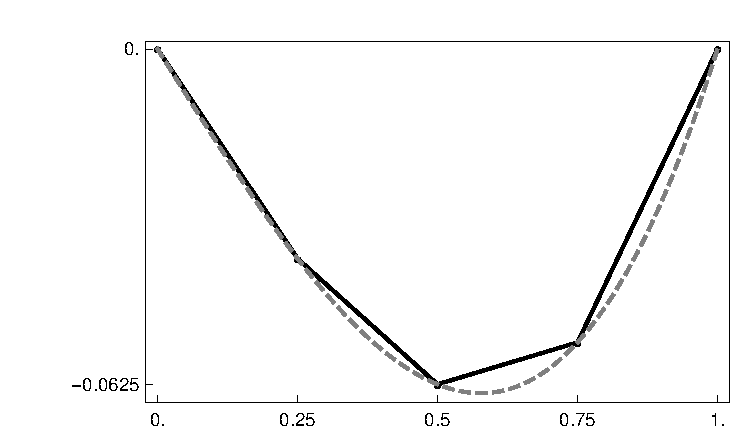
\includegraphics[width=\textwidth]{img/g3.pdf}
                \caption{Scaled: Green's functions}
                \label{g3}
            \end{subfigure}
            \begin{subfigure}{.49\textwidth}\centering
                \begin{tabular}{rl}
                    blue & \( G_0(x) \)  \\
                    orange & \( G(x,1/4) \) \\
                    green & \( G(x,1/2) \) \\
                    red & \( G(x,3/4) \) \\
                    purple & \( G_1(x) \) \\
                    black & linear combination \\
                    grey & actual solution
                \end{tabular}
                \caption{legend}
            \end{subfigure}
        \end{figure}



\end{enumerate}



\end{solution}

\begin{problem}[Problem 2 (Another way of analyzing the error using Green's functions)]
 The {\em composite trapezoid rule} for integration approximates the integral from \(a\) to \(b\) of a function \(g\) by dividing the interval into segments of length \(h\) and approximating the integral over each segment by the integral of the linear function that matches \(g\) at the endpoints of the segment. (For \(g > 0\), this is the area of the trapezoid with height \(g( x_j )\) at the left endpoint \(x_j\) and height \(g( x_{j+1} )\) at the right endpoint \(x_{j+1}\).)  Letting
\(h = (b-a)/(m+1)\) and \(x_j = a + jh\), \(j = 0,1, \ldots , m, m+1\):
\[
\int_a^b g(x)\,dx \approx  h \sum_{j=0}^m \frac{g( x_j )+g( x_{j+1} )}{2} 
     =  h \left[ \frac{g( x_0 )}{2} + \sum_{j=1}^m g( x_j ) + 
                   \frac{g( x_{m+1} )}{2} \right] .
\]

\begin{enumerate}
    \item[(a)] Assuming that \(g\) is sufficiently smooth, show that the error in the composite trapezoid rule approximation to the integral is \(O( h^2 )\). [Hint:  Show that the error on each subinterval is \(O( h^3 )\).]

    \item[(b)] Recall that the true solution of the boundary value problem \(u'' (x) = f(x)\), \(u(0) = u(1) = 0\) can be written as
\begin{equation}
u(x) = \int_0^1 f( \bar{x} ) G(x; \bar{x} )\,d \bar{x} , \label{1}
\end{equation}
where \(G(x; \bar{x})\) is the Green's function corresponding to \(\bar{x}\).  The finite difference approximation \(u_i\) to \(u( x_i )\), using the centered finite difference scheme in (2.43), is
\begin{equation}
u_i = h \sum_{j=1}^m f( x_j ) G( x_i ; x_j ) ,~~i=1, \ldots , m . \label{2}
\end{equation}
Show that formula (\ref{2}) is the trapezoid rule approximation to the integral in (\ref{1}) when \(x = x_i\), and conclude from this that the 
error in the finite difference approximation is \(O( h^2 )\) at each node \(x_i\). [Recall:  The Green's function \(G( x ; x_j )\) has a {\em discontinuous} derivative at \(x = x_j\).  Why does this not degrade the accuracy of thecomposite trapezoid rule?]
\end{enumerate}
\end{problem}

\begin{solution}[Solution]

\begin{enumerate}
    \item[(a)] Since \( g \) is sufficiently smooth, it is continuous and therefore has antiderivative \( G \) on \( (a,b) \).

        Let \( x=x_j \) for some \( j=0,1,\ldots, m \). We consider the error in using a single trapezoid to approximate the integral of the function on the interval \( (x,x+h) = (x_j,x_{j+1}) \).

        Expand \( G(x+h) \) about \( x \) as,
        \begin{align*}
            G(x+h) &= G(x) + G'(x)h + G''(x) \dfrac{h^2}{2!} + G'''(x) \dfrac{h^3}{3!} + \mathcal{O}(h^4) \\
            &= G(x) + g(x)h + g'(x) \dfrac{h^2}{2!} + g''(x) \dfrac{h^3}{3!}+\mathcal{O}(h^4)
        \end{align*}

        By the Fundamental Theorem of Calculus we then have,
        \begin{align*}
            \int_{x}^{x+h}g(t)dt = G(x+h) - G(x) = g(x)h + g'(x) \dfrac{h^2}{2!} + g''(x) \dfrac{h^3}{3!} + \mathcal{O}(h^4)
        \end{align*}

        Now expand \( g(x+h) \) about \( x \) as,
        \begin{align*}
            g(x+h) &= g(x) + g'(x)h + g''(x) \dfrac{h^2}{2!} + \mathcal{O}(h^3)
        \end{align*}

        The trapezoid approximation on the interval \( (x,x+h) \) is then,
        \begin{align*}
            \dfrac{h}{2}[g(x)+g(x+h)] &=
            \dfrac{h}{2}\left[2g(x) + g'(x)h + g''(x) \dfrac{h^2}{2!} + \mathcal{O}(h^3) \right] \\
            &= g(x) h + g'(x) \dfrac{h^2}{2} + g''(x) \dfrac{h^3}{2\cdot 3!} + \mathcal{O}(h^4)
        \end{align*}

        Thus, the error for a single interval of width \( h \) is,
        \begin{align*}
            \left( \int_{x}^{x+h}g(t)dt \right) - \dfrac{h}{2}[g(x)+g(x+h)] &=
            g''(x) \dfrac{h^3}{3!} - g''(x) \dfrac{h^3}{2\cdot 3!} + \mathcal{O}(h^4) = g''(x) \dfrac{h^3}{12} + \mathcal{O}(h^4)
        \end{align*}

        This proves that on an interval of width \( h \), the trapezoid rule has an error order \( h^3 \).

        To approximate the integral on the interval \( (a,b) \) we add up the results of \( m+1 = (b-a)/h \) trapezoid approximations for intervals of width \( h \). The total error is then at most,
        \begin{align*}
            (m+1) \left( \max_{x\in(a,b)} g''(x) \dfrac{h^3}{12} + \mathcal{O}(h^4) \right) = \mathcal{O}(h^2) \tag*{\qed}
        \end{align*}


    \item[(b)]
        Suppose \( f \) is ``sufficiently smooth''. Then \( g(\bar{x}):=f(\bar{x})G(x;\bar{x}) \) is piecewise ``sufficiently smooth'', with a possible discontinuity in some derivative of \( g(\bar{x}) \) at \( \bar{x} = x \) (since \( G(x;\bar{x}) \) is analytic except at \( \bar{x} = x \)).

        Our above analysis only requires that the function be smooth on the interval \( (x,x+h) \) for the error to be \( \mathcal{O}(h^3) \). 
        
        Thus, if \( x = x_i \), the discontinuity in \( g(\bar{x}) \) will be at one of the partition points of \( (0,1) \), so the analysis above is still applicable.

        %The Greens functions have discontinuities at \( x_j \), which will be the endpoints of our individual trapezoid approximations if we start at \( x_i \). Thus, within each interval \( (x_k,x_{k+1}) \) the approximation will be \( \mathcal{O}(h^3) \) so the total approximation will be \( \mathcal{O}(h^2) \). In short, given that we choose the partition of \( (a,b) \) such that the partition points are the only non-smooth points of \( g(x) \), the trapezoid approximation error bounds above are still applicable.

        Using the definition of the trapezoid rule,
        where \( x_j = jh \) and \( h=1/(m+1) \), we have
        \begin{align*}
            u(x) = \int_{0}^{1} f(\bar{x})G(x;\bar{x}) d\bar{x}
            \approx
            h \left[ \dfrac{f(x_0)G(x;x_0)}{2} + \sum_{j=1}^{m}f(x_j)G(x;x_j) + \dfrac{f(x_{m+1})G(x;x_{m+1})}{2} \right]
        \end{align*}

        Note that \( G(x,x_0) = 0(1-0) = 0 \) and \( G(x,x_{m+1}) = 1(1-1) = 0 \). Thus, at \( x=x_i \),
        \begin{align*}
            u(x_i) \approx h \sum_{j=1}^{m}f(x_j)G(x_i;x_j) 
        \end{align*}

        In particular, since the trapezoid approximation is equal to \( u(x) \) up to order \( h^2 \) for any \( x \), 
        \begin{align*}
            u(x_i) - h \sum_{j=1}^{m}f(x_j)G(x_i;x_j) = \mathcal{O}(h^2) \tag*{\qed}
        \end{align*}

\end{enumerate}

\end{solution}

\begin{problem}[Problem 3 (Green's function with Neumann boundary conditions)]
\begin{enumerate}
    \item[(a)] Determine the Green's functions for the two-point boundary value problem \(u''(x) = f(x)\) on \(0<x<1\) with a Neumann boundary condition at \(x=0\) and a Dirichlet condition at \(x=1\), i.e, find the function \(G(x,\bar x)\) solving
\[
u''(x) = \delta(x-\bar x), \quad u'(0)=0, \quad u(1)=0
\]
and the functions \(G_0(x)\) solving
\[
u''(x) = 0, \quad u'(0)=1, \quad u(1)=0
\]
and \(G_1(x)\) solving
\[
u''(x) = 0, \quad u'(0)=0, \quad u(1)=1.
\]
    \item[(b)] Using this as guidance, find the general formulas for the elements of the inverse of the matrix in equation (2.54).  Write out the \(5\times 5\) matrices \(A\) and \(A^{-1}\) for the case \(h=0.25\).
\end{enumerate}
\end{problem}

\begin{solution}[Solution]

\begin{enumerate}
    \item[(a)] 
        Integrating once yields a solution which is piecewise constant with a single discontinuity at \( x=\bar{x} \). Moreover, since the integral over an interval containing the delta function is equal to one, the jump at this discontinuity must be one. We are given the condition \( u'(0) = 0 \) so,
        \begin{align*}
            G'(x;\bar{x}) = \begin{cases}
                0 & 0 \leq x\leq \bar{x} \\
                1 & \bar{x} \leq x \leq 1
            \end{cases}
        \end{align*}

        Integrating again yields a piecewise linear function with a discontinuity in the derivative at \( x=\bar{x} \).
        That is,
        \begin{align*}
            G(x;\bar{x}) = \begin{cases}
                c & 0 \leq x \leq \bar{x} \\
                x + d & \bar{x} \leq x \leq 1
            \end{cases}
        \end{align*}
        
        Since the function is continuous we have, \( c = \bar{x} + d \). Moreover, we require \( u(1) = 0 \) which forces \( d=-1 \). Thus,
        \begin{align*}
            G(x;\bar{x}) = \begin{cases}
                \bar{x}-1 & 0 \leq x \leq \bar{x} \\
                x-1 & \bar{x} \leq x \leq 1
            \end{cases}
        \end{align*}

        
        By inspection it is clear that,
        \begin{align*}
            G_0(x) = x-1 && G_1(x) = 1
        \end{align*}
    \item[(b)]
        We have,
        \begin{align*}
            \dfrac{1}{h^2}
            \left[\begin{array}{rrrrr}
                -h & h \\
                1 & -2 & 1 \\
                & \ddots & \ddots & \ddots \\
                & & 1 & -2 & 1 \\
                & & & 0 & h^2 \\
            \end{array}\right]
            \left[\begin{array}{c}
                U_0 \\ U_1 \\ \vdots \\ U_m \\ U_{m+1}
            \end{array}\right]
            =
            \left[\begin{array}{c}
                \alpha \\ f(x_1) \\ \vdots \\ f(x_m) \\ \beta 
            \end{array}\right]
%            \left[\begin{array}{c}
 %               1 \\ f(x_1) \\ f(x_2) \\ f(x_3) \\ 0 
  %          \end{array}\right]
        \end{align*}

        We use the Greens functions derived above to write the inverse. 

        In the first and last columns we have,
        \begin{align*}
            B_{i,0} = x_i - 1
            && 
            B_{i,m+1} = 1
        \end{align*}

        In the middle columns we have,
        \begin{align*}
            B_{i,j} = hG(x_i;x_j) = \begin{cases}
                h(x_j-1) & i = 0,1,...,j \\
                h(x_i-1) & i = j,j+1, ..., m+1
            \end{cases}
        \end{align*}

       Thus, when \( h=1/4 \),
        \begin{align*}
            A = 
            \left[\begin{array}{rrrrr}
                -4 & 4  \\
                16 & -32 & 16 \\
                & 16 & -32 & 16 \\
                && 16 & -32 & 16 \\
                &&&&  1
            \end{array}\right]
        \end{align*}

        Again we have,
        \begin{align*}
            x_0 = 0 && x_1 = 1/4 && x_2 = 2/4 && x_3 = 3/4 && x_4 = 1
        \end{align*}
       

        Thus,
        \begin{align*}
            B = 
            \left[\begin{array}{rrrrr}
                x_0-1 & h(x_1-1) & h(x_2-1) & h(x_3-1) & 1 \\
                x_1-1 & h(x_1-1) & h(x_2-1) & h(x_3-1) & 1 \\
                x_2-1 & h(x_2-1) & h(x_2-1) & h(x_3-1) & 1 \\
                x_3-1 & h(x_3-1) & h(x_3-1) & h(x_3-1) & 1 \\
                x_4-1 & h(x_4-1) & h(x_4-1) & h(x_4-1) & 1
            \end{array}\right]
            =
            \left[\begin{array}{rrrrr}
                -1   & -3/16 & -1/8  & -1/16 & 1 \\
                -3/4 & -3/16 & -1/8  & -1/16 & 1 \\
                -1/2 & -1/8  & -1/8  & -1/16 & 1 \\
                -1/4 & -1/16 & -1/16 & -1/16 & 1 \\
                0    & 0     & 0     & 0     & 1 \\
            \end{array}\right]
        \end{align*}

        We easily verify that \( B=A^{-1} \) using Mathematica.

\end{enumerate}


\end{solution}

\begin{problem}[Problem 4 (Solvability condition for Neumann problem)]
Determine the null space of the matrix \(A^T\), where \(A\) is given in equation (2.58), and verify that the condition (2.62) must hold for the linear system to have solutions.
\end{problem}

\begin{solution}[Solution]

We have,
\begin{align*}
    A^T =
    \left[\begin{array}{rrrrrrr}
        -h & 1 \\
        h & -2 & 1 \\
        & 1 & -2 & 1 \\
        && 1 & -2 & 1 \\
        &&& \ddots & \ddots & \ddots \\
        &&&& 1 & -2 & h \\
        &&&&& 1 & -h
    \end{array}\right]
\end{align*}

Supposed \( x\in\ker A^T \). Then, multiplying by \( h^2 \) for simplicity,
\begin{align*}
    0 = h^2A^Tx = 
    \left[\begin{array}{rrrrrrr}
        -h & 1 \\
        h & -2 & 1 \\
        & 1 & -2 & 1 \\
        && 1 & -2 & 1 \\
        &&& \ddots & \ddots & \ddots \\
        &&&& 1 & -2 & h \\
        &&&&& 1 & -h
    \end{array}\right]
    \left[\begin{array}{r}x_0 \\ x_1 \\ x_2 \\ x_3 \\ \vdots \\ x_m \\ x_{m+1}\end{array}\right]
    =
    \left[\begin{array}{r}
        -hx_0 +x_1 \\ 
        hx_0-2x_1+x_2 \\
        x_1-2x_2+x_3 \\
        x_2-2x_3+x_4 \\
        \vdots \\
        x_{m-1}-2x_m+hx_{m+1} \\
        x_m - hx_{m+1}
    \end{array}\right]
\end{align*}

Thus,
\begin{align*}
    x_1 &= hx_0  \\
    x_2 &= 2x_1 - hx_0 = hx_0 \\
    x_3 &= 2x_2 - x_1 = hx_0 \\
    x_4 &= 2x_3 - x_2 = hx_0 \\
    &\vdots \\
    x_{m} &= 2x_{m-1}-x_{m-2} = hx_0 \\
    x_{m+1} &= (2x_m-x_{m-1})/h = x_0 \\
    x_{m+1} &= x_m/h = x_0
\end{align*}

The null space of \( A^T \) is then, \( \operatorname{span}\{[1,h,h,\ldots,h,1]\} \)

Recall that the range of \( A \) is perpendicular to the null space of \( A^T\). Clearly \( AU = F \) has a solution if and only if \( F\in\operatorname{range}A = (\operatorname{null}A^T)^\perp \).

That is, the system \( AU = F \) has solutions if and only if \( F \) is orthogonal to the null space of \( A^T \). 

Since \( \operatorname{null}A^T \) is spanned by \( y=[1,h,h,\ldots,h,1] \) every vector has the form \( cy \) for some \( c\in\RR \). It is then sufficient to show that \( y^TF = 0 \) as this will imply \( (cy)^TF = 0 \) for any vector \( cy \in \operatorname{null}A^T \).

Then, \( F \) is orthogonal to \( y \) (and \( \operatorname{null}A^T \)) if and only if,
\begin{align*}
    0 = y^TF = 1\left(\sigma_0 + \dfrac{h}{2}f(x_0) \right) + h(f(x_1)) + h(f(x_2)) + \cdots +  h(f(x_m)) + 1 \left( -\sigma_1 + \dfrac{h}{2}f(x_{m+1})\right)
\end{align*}

Equivalently, moving \( \sigma_0 \) and \( -\sigma_1 \) to the other side, and using sum notation to condense the middle terms,
\begin{align*}
    \dfrac{h}{2}f(x_0) + h\sum_{i=1}^{m}f(x_i) + \dfrac{h}{2}f(x_{m+1}) = \sigma_1 - \sigma_0
\end{align*}

This is exactly condition 2.62. \qed

\end{solution}

\begin{problem}[Problem 5 (Symmetric tridiagonal matrices)]
\begin{enumerate}
    \item[(a)] Consider the {\bf Second approach} described on p.~31 for dealing with a Neumann boundary condition.  If we use this technique to approximate the solution to the boundary value problem \(u'' (x) = f(x)\), \(0 \leq x \leq 1\), \(u' (0) = \sigma\), \(u(1) = \beta\), then the resulting linear system \(A {\bf u} = {\bf f}\) has the following form:
\[
    \frac{1}{h^2} \left[ \begin{array}{ccccc}
-h & h  &        &        &      \\
1  & -2 & 1      &        &      \\
   & 1  & \ddots & \ddots &      \\
   &    & \ddots & \ddots & 1    \\
   &    &        & 1      & -2 \end{array} \right]
        \left[ \begin{array}{c} u_0 \\ u_1 \\ \vdots \\ u_{m-1} \\ u_{m} \end{array} 
    \right] =
        \left[ \begin{array}{c} \sigma + (h/2) f( x_0 ) \\ f( x_1 ) \\ \vdots \\ 
        f( x_{m-1} ) \\ f( x_m ) - \beta / h^2 \end{array} \right]
\]
Show that the above matrix is similar to a symmetric tridiagonal matrix via a {\em diagonal} similarity transformation; that is, there is a diagonal matrix \(D\) such that \(D A D^{-1}\) is symmetric.
    \item[(b)] Consider the {\bf Third approach} described on pp.~31-32 for dealing with a Neumann boundary condition.  [{\bf Note:} If you have an older edition of the text, there is a typo in the matrix (2.57) on p.~32.  There should be a row above what is written there that has entries \(\frac{3}{2} h\), \(-2h\), and \(\frac{1}{2} h\) in columns \(1\) through \(3\) and \(0\)'s elsewhere.  I believe this was corrected in newer editions.]  
Show that if we use that first equation (given at the bottom of p. 31) to eliminate \(u_0\) and we also eliminate \(u_{m+1}\) from the equations by setting it equal to \(\beta\) and modifying the right-hand side vector accordingly, then we obtain an \(m\) by \(m\) linear system \(A {\bf u} = {\bf f}\), where \(A\) is similar to a symmetric tridiagonal matrix via a diagonal similarity transformation.
\end{enumerate}
\end{problem}

\begin{solution}[Solution]
\begin{enumerate}
    \item[(a)] The only non-symmetric entries are the (0,1) and (1,0) entires. We then expect \( D \) to be mostly the identity except the first entry. Pick, \( D = \operatorname{diag}([1/\sqrt{h}, 1, 1, \ldots, 1]) \). Then, \( D^{-1} = \operatorname{diag}([\sqrt{h},1,1,\ldots,1]) \) so clearly,
        \begin{align*}
            DAD^{-1} = 
            \dfrac{1}{h^2}
            \left[\begin{array}{rrrrr}
                -h & \sqrt{h}    \\
                \sqrt{h}  & -2 & 1 \\
                & 1 & \ddots & \ddots    \\
                && \ddots & \ddots & 1    \\
                &&& 1  & -2 
            \end{array}\right] 
        \end{align*}
\iffalse
        \begin{align*}
            DAD^{-1} &=  
            \left[\begin{array}{rrrrr}
                1/\sqrt{h} \\
                & 1 \\
                && 1 \\
                &&& \ddots \\
                &&&&1 
            \end{array}\right]
            \left[\begin{array}{rrrrr}
                -h & h    \\
                1  & -2 & 1 \\
                & 1 & \ddots & \ddots    \\
                && \ddots & \ddots & 1    \\
                &&& 1  & -2 
            \end{array}\right]
            \left[\begin{array}{rrrrr}
                \sqrt{h} \\
                & 1 \\
                && 1 \\
                &&& \ddots \\
                &&&&1 
            \end{array}\right]
            \\&=
            \left[\begin{array}{rrrrr}
                -h & \sqrt{h}    \\
                \sqrt{h}  & -2 & 1 \\
                & 1 & \ddots & \ddots    \\
                && \ddots & \ddots & 1    \\
                &&& 1  & -2 
            \end{array}\right]
        \end{align*}
\fi
    \item[(b)]
        Suppose \( U_{m+1} = \beta \), along with the boundary equation,
        \begin{align*}
            \dfrac{1}{h} \left( \dfrac{3}{2}U_0-2U_1+\dfrac{1}{2}U_2 \right) = \sigma \tag{*}
        \end{align*}
        
        We then have the system,
        \begin{align*}
            \dfrac{1}{h^2}
            \left[\begin{array}{cccccc}
                \frac{3h}{2} & -2h & \frac{h}{2} \\
                1 & -2 & 1 \\
                & 1 & -2 & 1 \\
                && \ddots & \ddots & \ddots \\
                &&& 1 & -2 & 1 \\
                &&&& 0 & h^2
            \end{array}\right]
            \left[\begin{array}{c}
                U_0 \\ U_1 \\ U_2 \\ \vdots \\ U_m \\ U_{m+1}
            \end{array}\right]
            =
            \left[\begin{array}{c}
                \sigma \\ f(x_1) \\ f(x_2) \\ \vdots \\ f(x_m) \\ \beta
            \end{array}\right]
        \end{align*}

        We eliminate \( U_0 \) by subtracting \( 2/3h \) times row zero from row one, and we eliminate \( U_{m+1} \) by subtracting \( 1/h^2 \) times row \( m+1 \) from row \( m \). Thus,
        \begin{align*}
            \dfrac{1}{h^2}
            \left[\begin{array}{ccccccc}
                \frac{3h}{2} & -2h & \frac{h}{2} \\
                0 & -\frac{2}{3} & \frac{2}{3} \\
                & 1 & -2 & 1 \\
                && \ddots & \ddots & \ddots \\
                &&& 1 & -2 & 1 \\
                &&&& 1 & -2 & 0 \\
                &&&&& 0 & h^2
            \end{array}\right]
            \left[\begin{array}{c}
                U_0 \\ U_1 \\ U_2 \\ \vdots \\ U_{m-1} \\ U_m \\ U_{m+1}
            \end{array}\right]
            =
            \left[\begin{array}{c}
                \sigma \\ f(x_1) - \frac{2}{3h} \sigma \\ f(x_2) \\ \vdots \\ f(x_{m-1}) \\ f(x_m) - \frac{1}{h^2}\beta \\ \beta
            \end{array}\right]
        \end{align*}


        Thus, given equation (*) and \( U_{m+1} = \beta \) we have the \( m\times m \) system,
        \begin{align*}
            \dfrac{1}{h^2}
            \left[\begin{array}{ccccccc}
                -\frac{2}{3} & \frac{2}{3} \\
                1 & -2 & 1 \\
                & \ddots & \ddots & \ddots \\
                && 1 & -2 & 1 \\
                &&& 1 & -2
            \end{array}\right]
            \left[\begin{array}{c}
                U_1 \\ U_2 \\ \vdots \\ U_{m-1} \\ U_m
            \end{array}\right]
            =
            \left[\begin{array}{c}
                f(x_1) - \frac{2}{3h}\sigma \\ f(x_2) \\ \vdots \\ f(x_{m-1}) \\ f(x_m)  \frac{1}{h^2}\beta
            \end{array}\right]
        \end{align*}

         Pick, \( D = \operatorname{diag}([\sqrt{3/2}, 1, 1, \ldots, 1]) \). Then, \( D^{-1} = \operatorname{diag}([\sqrt{2/3},1,1,\ldots,1]) \) so clearly,
        \begin{align*}
            DAD^{-1} = 
            \dfrac{1}{h^2}
            \left[\begin{array}{ccccc}
                -\frac{2}{3} & \sqrt{\frac{2}{3}}    \\
                \sqrt{\frac{2}{3}}  & -2 & 1 \\
                & 1 & \ddots & \ddots    \\
                && \ddots & \ddots & 1    \\
                &&& 1  & -2 
            \end{array}\right] 
        \end{align*}

\end{enumerate}

\end{solution}
\end{document}
